%!TEX root = main.tex
\add{
\subsection{Cyclic Queries}
\label{sec:cyclic_queries}
Our framework supports arbitrary conjunctive queries. Whereas for an acyclic join query the size of each view is asymptotically upper-bounded by the size of the query result, for a cyclic query views may be larger in size than the 
query result. 
%This increase in space may however enable faster view maintenance.
In prior work~\cite{FIVM:SIGMOD:2018}, we show how to reduce the size of intermediate views
for cyclic queries  by extending view trees with indicator projections~\cite{FAQ:PODS:2016}.  Such projections have no effect on the query result but can constrain view definitions (e.g., create cycles) and bring asymptotic savings in space and time. 

}

\begin{example}\label{ex:triangle_query_ivm}
We consider the triangle query: 
%over the ring $\mathbb{Z}$:
% 
$$
\VIEW[~]{Q_{\vartriangle}} = \VSUM_{A}\VSUM_{B}\VSUM_{C} \VIEW[A,B]{R} \VPROD \VIEW[B,C]{S} \VPROD \VIEW[C,A]{T} 
$$

Figure~\ref{fig:triangle_hypergraph_viewtree} shows the hypergraph of $Q_{\vartriangle}$ and the view tree constructed for the variable order $A-B-C$ by placing each relation directly under its lowest variable. We assume all {relations} are of size $\bigO{N}$. Computing the triangle query from scratch using a worst-case optimal join algorithm takes $\bigO{N^{3/2}}$ time~\cite{Ngo:SIGREC:2013}.

In the given view tree (without the view in red), we first join $\VIEW{S}$ and $\VIEW{T}$ and then marginalize out $C$.
This view at node $C$ may contain $\bigO{N^2}$ pairs of $(A,B)$ values, which is larger than the worst-case size $\bigO{N^{3/2}}$. 
However, by materializing the view at $C$, we enable single-tuple updates to $R$ in constant time; single-tuple updates to other relations take $\bigO{N}$ time.

To avoid the large intermediate result at variable $C$, we can change the view tree by placing the relation $R$ under variable $C$. Then, joining all three relations at node $C$ takes $\bigO{N^{3/2}}$ time. Updates to any relation now cause recomputation of a $3$-way join, like in first-order IVM. For single-tuple updates, recomputing deltas takes $\bigO{N}$ as only two of the three variables are bound to constants. In contrast, the first approach trades off space for time: We need $\bigO{N^2}$ space but then support $\bigO{1}$ updates to one of the three relations.
\punto
\end{example}


\begin{figure}\centering
  \begin{tabular}[c]{l@{~~~}l}  
    \begin{minipage}[b]{3cm}
      \scalebox{0.9}{
      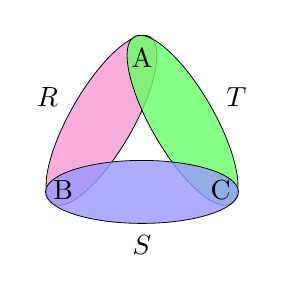
\begin{tikzpicture}[scale=0.5]
        \node at (-2.4, -2) (r) {$R$};
        \node at (2.4, -2) (r) {$T$};
        \node at (0, -5.75) (r) {$S$};
        \draw[rotate=60,line width=0.1mm,fill opacity=0.8,fill=magenta!40] (-2.75,-0.4) ellipse (2.45cm and 0.8cm);
       \draw[rotate=-60,line width=0.1mm,fill opacity=0.8,fill=green!60] (2.75,-0.4) ellipse (2.45cm and 0.8cm);
        \draw[rotate=0,line width=0.1mm,fill opacity=0.8,fill=blue!40] (0,-4.4) ellipse (2.45cm and 0.8cm);
        \node at (0, -1) (A) {A};
        \node at (-2, -4.35) (B) {B};
        \node at (2, -4.35) (C) {C};
      \end{tikzpicture}
      }
      \vspace{2mm}
    \end{minipage}
    &
    \begin{minipage}[b]{5cm}
      \scalebox{0.9}{
      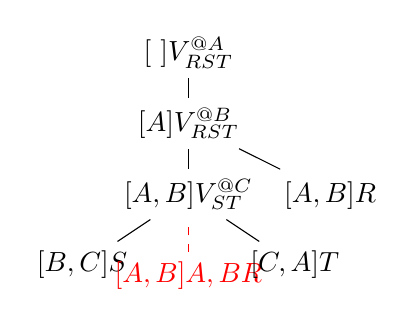
\begin{tikzpicture}[xscale=0.9,yscale=0.9]
        \node at (0, 0) (A) {$\VIEW[~]{V^{@A}_{RST}}$};
        \node at (0, -1) (B) {$\VIEW[A]{V^{@B}_{RST}}$} edge[-] (A);
        \node at (0, -2) (C) {$\VIEW[A,B]{V^{@C}_{ST}}$} edge[-] (B);

        \node at (2, -2) (R) {$\VIEW[A,B]{R} \makebox[0pt][l]{$\phantom{\VIEW[A,B]{V^{@C}}}$} $} edge[-] (B);
        \node at (-1.5, -3) (S) {$\VIEW[B,C]{S}$} edge[-] (C);
        \node[color=red] at (-0, -3.15) (S) {$\VIEW[A,B]{\displaystyle\VEXISTS{A,B}{R}}$} edge[red,dashed] (C);
        \node at (1.5, -3) (T) {$\VIEW[C,A]{T}$} edge[-] (C);
      \end{tikzpicture}
  }    
    \end{minipage}
    \end{tabular}
    % \vspace*{-1em}
\caption{(left) Hypergraph of the triangle query $Q_{\vartriangle}$; (right) View tree for the variable order $A - B - C$ with an indicator projection $\exists_{A,B}\VIEW{R}$.}
\label{fig:triangle_hypergraph_viewtree}
% \vspace*{2em}
\end{figure}


\nop{
\begin{figure}\centering
  \begin{tabular}[c]{@{}l@{~}l@{}}  
    \begin{minipage}[b]{2.3cm}
      \hspace*{-4mm}
      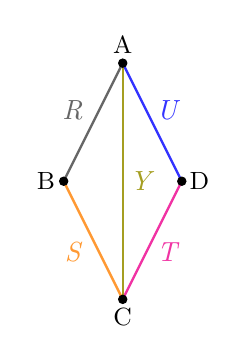
\begin{tikzpicture}[xscale=0.75,yscale=0.75]

        \draw[thick,darkgray!80,line width=0.3mm] (0,0) -- (-1,-2);
        \draw[thick,blue!80,line width=0.3mm] (0,0) -- (1,-2);        
        \draw[thick,orange!80,line width=0.3mm] (-1,-2) -- (0,-4);
        \draw[thick,magenta!80,line width=0.3mm] (1,-2) -- (0,-4);
        \draw[thick,olive!80,line width=0.3mm] (0,0) -- (0,-4);

        \draw[fill=black] (0,0) circle (0.7mm);
        \draw[fill=black] (-1,-2) circle (0.7mm);
        \draw[fill=black] (1,-2) circle (0.7mm);
        \draw[fill=black] (0,-4) circle (0.7mm);

        \node at (0,0.3) {\small A};
        \node at (-1.3,-2) {\small B};        
        \node at (1.3,-2) {\small D};
        \node at (0.0,-4.3) {\small C};

        \node at (-0.85, -0.8) (r) {\color{darkgray!80}\it R};
        \node at (0.75, -0.8) (r) {\color{blue!80}\it U};
        \node at (-0.85, -3.2) (r) {\color{orange!80}\it S};
        \node at (0.75, -3.2) (r) {\color{magenta!80}\it T};
        \node at (0.3, -2) (r) {\color{olive!80}\it Y};
      \end{tikzpicture}
      \vspace{3mm}
    \end{minipage}
    &
    \begin{minipage}[b]{5.5cm}
      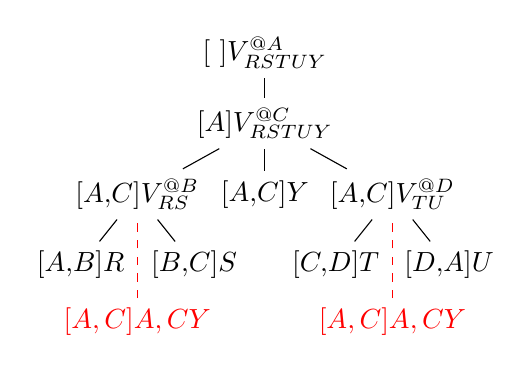
\begin{tikzpicture}[xscale=0.9,yscale=0.9]
        \node at (0, 0) (A) {$\VIEW[~]{V^{@A}_{RSTUY}}$};
        \node at (0, -1) (C) {$\VIEW[A]{V^{@C}_{RSTUY}}$} edge[-] (A);
        \node at (-1.8, -2) (B) {$\VIEW[A,\!C]{V^{@B}_{RS}}$} edge[-] (C);
        \node at (0, -2) (Y) {$\VIEW[A,\!C]{Y}$} edge[-] (C);
        \node at (1.8, -2) (D) {$\VIEW[A,\!C]{V^{@D}_{TU}}$} edge[-] (C);
        \node at (-2.6, -3) (R) {$\VIEW[A,\!B]{R}$} edge[-] (B);
        \node at (-1.0, -3) (S) {$\VIEW[B,\!C]{S}$} edge[-] (B);
        \node at (1.0, -3) (T) {$\VIEW[C,\!D]{T}$} edge[-] (D);
        \node at (2.6, -3) (U) {$\VIEW[D,\!A]{U}$} edge[-] (D);

        \node[color=red] at (-1.8, -3.8) (P1) {$\VIEW[A,C]{\VEXISTS{A,C}Y}$} edge[red,dashed] (B);
        \node[color=red] at (1.8, -3.8) (P2) {$\VIEW[A,C]{\VEXISTS{A,C}Y}$} edge[red,dashed] (D);
      \end{tikzpicture}
    \end{minipage}
    \end{tabular}
\caption{\label{fig:cyclic_hypergraph_viewtree}(left) Hypergraph of the cyclic query $Q_{\boxslash}$; (right) View tree for the variable order $A - C - \{ B, D \}$ with indicator projections (in red).}
\vspace{-1em}
\end{figure}
}

The above example demonstrates how placing a relation under a different node in a view tree can create a cycle of relations and constrain the size of a view. This strategy, however, might not be always feasible or efficient: One relation might form multiple cycles of relations in different parts of a view tree -- for example, in the cyclic $4$-loop
 query $\VIEW[~]{Q_{\boxslash}}$ $=$ 
 $\VSUM_{A}\VSUM_{B}\VSUM_{C} \VSUM_{D}$ $\VIEW[A,B]{R}\VPROD \VIEW[B,C]{S} \VPROD \VIEW[C,D]{T}
 \VPROD \VIEW[D,A]{U} \VPROD \VIEW[A,C]{W}$ the chord relation $\VIEW{W}$ is part of two triangle subqueries. Since this relation cannot be duplicated in multiple subtrees (for correctness reasons so as to avoid multiplying the same payload several times instead of using it once), one would have to evaluate these subqueries in sequence, which yields a view tree that is higher and more expensive to maintain. 

\paragraph{\textbf{Indicator Projections.}}
Instead of moving relations in a view tree, we extend the tree with indicator projections that identify the active domains of these relations~\cite{FAQ:PODS:2016}. Such projections have no effect on the query result but can constrain view definitions (e.g., create cycles) and bring asymptotic savings in space and time. 

We define a new unary operation $\VEXISTS{\mathcal{A}}{\VIEW{R}}$ that, given a relation $\VIEW{R}$ over schema 
$\mathcal{S}$ with payloads from a ring $(\RING, \RINGPLUS, \RINGPROD, \RINGZERO, \RINGONE)$, and a set of attributes $\mathcal{A} \subseteq \mathcal{S}$, projects tuples from $\VIEW{R}$ with non-$\RINGZERO$ payload on $\mathcal{A}$ and assigns to these tuples the payload $\RINGONE$. 


\begin{definition}[Indicator Projection]
   For a relation R over schema $\calS$ and $\calA \subseteq \calS$, 
   the indicator projection $\VEXISTS{\mathcal{A}}{\VIEW{R}}$ is a relation over $\calA$ such that
   $\forall \vecnormal{t} \in \Dom(\calA)$:
\begin{align*}
  \left( \textstyle\VEXISTS{\mathcal{A}}{\VIEW{R}} \right)[\vecnormal{t}] = 
  \begin{cases} 
    \RINGONE & \exists\vecnormal{s} \in\Dom(\mathcal{S}), \vecnormal{s}\in \VIEW{R}, \vecnormal{t} = \pi_{\mathcal{A}}(\vecnormal{s})\\
    \RINGZERO & \text{otherwise}
  \end{cases}
\end{align*}
\end{definition}


\nop{
The delta rule for $\VEXISTS{\mathcal{A}}$ is $\delta(\VEXISTS{\mathcal{A}}{\VIEW{R}}) = \VEXISTS{\mathcal{A}}(\VIEW{R} + \delta{\VIEW{R}}) - \VEXISTS{\mathcal{A}}{\VIEW{R}}$. This rule recomputes the query twice, once to insert new contents and once to delete the old contents, which clearly defeats the purpose of incremental computation. Note that some tuples might be unaffected by a given update $\delta{\VIEW{R}}$, so inserting those tuples and deleting them again is wasted work.

We observe that $\delta(\VEXISTS{\mathcal{A}}{\VIEW{R}})$ might change in the output only those tuples from $\VEXISTS{\mathcal{A}}{\delta{\VIEW{R}}}$. We exploit this restriction to refine the delta rule as: $\delta(\VEXISTS{\mathcal{A}}{\VIEW{R}}) = \VEXISTS{\mathcal{A}}{\delta{\VIEW{R}}} \VPROD (\VEXISTS{\mathcal{A}}(\VIEW{R} + \delta{\VIEW{R}}) - \VEXISTS{\mathcal{A}}{\VIEW{R}})$.
}

Indicator projections may change with updates to input relations. For instance, adding a tuple with a 
new $\mathcal{A}$-value to $\VIEW{R}$ enlarges the result of $\VEXISTS{\mathcal{A}}\VIEW{R}$; similarly, deleting the last tuple with the given $\mathcal{A}$-value reduces the result. One change in the input may cause at most one change in the output: $|\delta{(\VEXISTS{\mathcal{A}}\VIEW{R})}| \le |\delta{\VIEW{R}}|$.

To facilitate the computation of $\delta{(\VEXISTS{\mathcal{A}}\VIEW{R})}$, we keep track of how many tuples with non-$\RINGZERO$ payloads project on each $\mathcal{A}$-value. For updating the payload of a tuple in $\VIEW{R}$ from $\RINGZERO$ to non-$\RINGZERO$ (or vice versa), we increase (decrease) the count corresponding to the given $\mathcal{A}$-value. If this count changes from $0$ to $1$ (meaning the $\mathcal{A}$-value is unique) or from $1$ to $0$ (meaning there are no more tuples with the $\mathcal{A}$-value), then $\delta{(\VEXISTS{\mathcal{A}}\VIEW{R})}$ contains a tuple of $\mathcal{A}$-values with the payload of $\RINGONE$ or $-\RINGONE$, respectively; otherwise, the delta is empty.

\begin{example}
Consider a relation $\VIEW{R}$ over schema $\{A,B\}$ and 
with payloads from a ring $(\RING, \RINGPLUS, \RINGPROD, \RINGZERO, \RINGONE)$. We want to maintain the result of the query $\VIEW[A]{Q} = \VEXISTS{A}\VIEW[A,B]{R}$. To compute $\VIEW[A]{\delta{Q}}$ for updates to $\VIEW{R}$ efficiently, we count the tuples from $\VIEW{R}$ with non-$\RINGZERO$ payloads for each $A$-value, denoted by $\VIEW[A]{CNT_{Q}}$. For example:
\begin{small}
\begin{align*}
  \begin{tabular}[t]{@{}l|@{~}c@{~}c@{~}c@{~}c@{}}
    $\VIEW{R}$ & A & B \\
    \midrule
    & $a_1$ & $b_1$ & $\to$ & $r_1$ \\
    & $a_1$ & $b_2$ & $\to$ & $r_2$ \\  
    & $a_2$ & $b_3$ & $\to$ & $r_3$ \\
  \end{tabular}
  \quad
  \begin{tabular}[t]{@{}l|@{~}c@{~}c@{~}c@{}}
    $\VIEW{CNT_{Q}}$ & A \\
    \midrule
    & $a_1$ & $\to$ & $2$ \\
    & $a_2$ & $\to$ & $1$ \\
  \end{tabular}
  \quad
  \begin{tabular}[t]{@{}l|@{~}c@{~}c@{~}c@{}}
    $\VIEW{Q}$ & A \\
    \midrule
    & $a_1$ & $\to$ & $\RINGONE$ \\
    & $a_2$ & $\to$ & $\RINGONE$ \\
  \end{tabular}
\end{align*}
\end{small}
where $r_1$, $r_2$, and $r_3$ are non-$\RINGZERO$ payloads from $\RING$.
% 
An update $\VIEW{\delta{R}} = \{ \tuple{a_1, b_2} \to -r_2 \}$ removes the tuple $\tuple{a_1,b_2}$ from $\VIEW{R}$, which in turn decreases $\VIEW[\text{$a_1$}]{CNT_{Q}}$ by $1$. Since there is still a tuple in $\VIEW{R}$ that projects on $a_1$, the result of $\VIEW{Q}$ remains unchanged. 
A subsequent update $\{ \tuple{a_1, b_1} \to -r_1 \}$ to $\VIEW{R}$ drops the count for $a_1$ to $0$, which triggers a change in the output, $\VIEW{\delta{Q}} = \{ \tuple{a_1} \to -\RINGONE \}$.
\punto
\end{example}


\begin{figure}[t]
	\centering
	\setlength{\tabcolsep}{3pt}
	\begin{tabular}[t]{@{}c@{}c@{}l@{}}
		\toprule
		\multicolumn{3}{c}{$indicators(\text{view tree } \tau)$ : view tree}   \\
		\midrule
		\multicolumn{3}{l}{\MATCH $\tau$:}                       \\
		\midrule
		\phantom{ab} & $\VIEW{R}(\calS))$ \hspace*{2.5em} & 

		  \RETURN $\VIEW{R}(\calS)$ \\
		\cmidrule{2-3} \\[-6pt]
		             &
		\begin{minipage}[t]{1.5cm}
			\vspace{-1.5em}
			\hspace*{-0.55cm}
			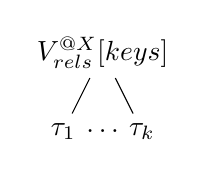
\begin{tikzpicture}[xscale=0.5, yscale=1]
				\node at (0,-2)  (n4) {$\VIEW{V_{rels}^{@X}}[keys]$};
				\node at (-1,-3)  (n1) {$\tau_1$} edge[-] (n4);
				\node at (0,-3)  (n2) {$\ldots$};
				\node at (1,-3)  (n3) {$\tau_k$} edge[-] (n4);
			\end{tikzpicture}
		\end{minipage}
		             &
		\begin{minipage}[t]{5.8cm}
			\vspace{-0.4cm}
			 \LET $\hat{\tau}_i = indicators(\tau_i)$ \ $\forall i\in[k]$ \\[0.5ex]
		          \LET $\calR $ be the set of all relation symbols  \\[0.5ex]
		           \LET $\calI = \{\VEXISTS{pk}\VIEW{R}\mid \VIEW{R} \in \calR \setminus \textsf{rels} \text{ and } \\[0.5ex]
		           \TAB\TAB\TAB\STAB pk = \sch(\VIEW{R}) \cap keys \neq \emptyset \}$ \\[0.5ex]
			 \LET $\{I_1, \ldots , I_{\ell}\} = \textsf{GYO}^*(\calI,\textsf{rels})$ \\[0.5ex] 
		  \RETURN $\left\{
				\begin{array}{@{~~}c@{~~}}
					\tikz {
						\node at (3.6,-1)  (n4) {$X$};
					        \node at (2.2,-1.75)  (n1) {$\hat{\tau}_1$} edge[-] (n4);
						\node at (2.65,-1.75)  (n2) {$\ldots$};
						\node at (3.2,-1.75)  (n3) {$\hat{\tau}_k$} edge[-] (n4);
						\node at (4.0,-1.75)  (n3) {$I_1$} edge[-] (n4);
						\node at (4.4,-1.75)  (n2) {$\ldots$};
						\node at (4.9,-1.75)  (n3) {$I_\ell$} edge[-] (n4);
					}
				\end{array}  \right.$
		\end{minipage}                                              \\[2.75ex]
		\bottomrule
	\end{tabular}
	\caption{Adding indicator projections to a view tree $\tau$. 
	Each view in $\tau$ gets as new children the indicator projections of relations that do not occur in the subtree rooted at the view  but form a cycle with those that occur. 
	$\textsf{GYO}^*$ is based on the GYO reduction~\cite{BeeriFMY83}.}
	\label{fig:indicator_projections_algo}
\end{figure}

\paragraph{\textbf{View Trees with Indicator Projections.}}
Figure~\ref{fig:indicator_projections_algo} gives an algorithm that traverses a given view tree 
recursively and extends it with indicator projections. At each view $\VIEW{V^{@X}_{rels}}$, the algorithm first computes a set 
$\calI$ of indicator projections for those relations that share common variables with $\VIEW{V^{@X}_{rels}}$ and 
do not appear in \textsf{rels}, hence do not take part 
in the view definition.
Then, it chooses from this set those indicator projections 
that form a cycle with the relations 
in the subtree rooted at $\VIEW{V^{@X}_{rels}}$. To achieve this,
it uses a variant of the \textsf{GYO} reduction~\cite{BeeriFMY83}.  
  Given the hypergraph formed by 
the hyperedges representing the indicator projections $\calI$ and the relations \textsf{rels}, 
\textsf{GYO} repeatedly applies two rules until it
reaches a fixpoint: (1) Remove a node that only appears in one hyperedge; (2) Remove a
hyperedge that is included in another hyperedge. If the result of \textsf{GYO} is a hypergraph with
no nodes and one empty hyperedge, then the input hypergraph is acyclic. Otherwise,
the input hypergraph is cyclic and the output of \textsf{GYO} is a hypergraph with cycles. The \textsf{GYO}
variant, dubbed $\textsf{GYO}^*$ in the procedure in Figure~\ref{fig:indicator_projections_algo}, returns the 
hyperedges that originated from the indicator
projections in $\calI$ and contribute to this non-empty output hypergraph. The chosen indicator
projections become children of $\VIEW{V^{@X}_{rels}}$.


In a view tree with indicator projections, changes in one relation may propagate along multiple leaf-to-root paths. We propagate them in sequence, that is, updates to one relation are followed by a sequence of updates to its indicator projections. 

\begin{example}
The algorithm from Figure~\ref{fig:indicator_projections_algo} extends the view tree of the triangle query with an indicator projection $\VEXISTS{A,B}\VIEW[A,B]{R}$ placed below the view $\VIEW{V^{@C}_{ST}}$. This view at $C$ is now a cyclic join of the three relations, which can be computed in $\bigO{N^{3/2}}$ time. The indicator projection also reduces the size of this view to $\bigO{N}$.

Single-tuple updates to $S$ and $T$ still take linear time; however, bulk updates of size $\bigO{N}$ can now be processed in $\bigO{N^{3/2}}$ time, same as reevaluation. Updates to $R$ might affect the indicator projection: If a single-tuple update $\VIEW{\delta{R}}$ causes no change in the projection, then incremental maintenance takes constant time; otherwise, joining a tuple $\delta({\VEXISTS{A,B}\VIEW{R}})$ with $\VIEW{S}$ and $\VIEW{T}$ at node $C$ takes linear time. Bulk updates $\VIEW{\delta{R}}$ of size $\bigO{N}$ can also be processed in $\bigO{N^{3/2}}$ time. We conclude that using indicator projections in this query takes the best of both approaches from Example~\ref{ex:triangle_query_ivm}, namely faster incremental maintenance and more succinct view representation.
\punto
\end{example}